\chapter{Optimizing patients travel}

\section{Context}

Cancer treatment delay is a problem in health systems worldwide, increasing
mortality for many types of cancers \cite{hanna_mortality_2020}, including
breast cancer \cite{caplan_delay_1992, williams_assessment_2015,
    pace_delays_2015}. Distance between patients residence and diagnosing hospitals
is among the factors causing these delays, especially for cancer types that are
hard to diagnose \cite{flytkjaer_virgilsen_cancer_2019}. While accessibility to
healthcare is growing, research found that 8.9\% of the global population (646
million people) could not reach healthcare within one hour if they had access to
motorized transport \cite{weiss_global_2020}. Thus, a non insignificant part of
the population might be exposed to lower prognosis.

The benefits of centralized healthcare have been debated. A centralized approach
often requires patients to travel far away from their home and their local
community hospitals \cite{woo_centralisation_2012}. Patients subject to longer
travels to reach a specialized hospital are likely to be affected by the travel
burden and separation from their social environment \cite{payne_impact_2000}. In
the debate between local versus centralized healthcare provision, there are
evidence of an association between travel distance and health outcomes
\cite{kelly_are_2016}. Unsurprisingly, travel to cancer treatment is
inconvenient for some patients and might even act as a barrier to treatment
\cite{payne_impact_2000}. Research also showed that patients who lived far from
hospitals and had to travel more than 50 miles had a more advanced stage at
diagnosis, lower adherence to encoded treatments, a worse prognosis, and a worse
quality of life \cite{ambroggi_distance_2015}. More research linked travel
burden with lower treatment compliance
\cite{dutta_evaluation_2013,guidry_transportation_1997}. The distance from the
hospital influences the choice of appropriate treatment by cancer patients. In
breast cancer, patients living farther from a radiation treatment facility more
often underwent mastectomy instead of breast conservative surgery
\cite{schroen_impact_2005,celaya_travel_2006,voti_treatment_2006,meden_relationship_2002,nattinger_relationship_2001,boscoe_geographic_2011}
or did not undergo radiotherapy after breast cancer surgery
\cite{satasivam_dilemma_2014,schroen_impact_2005,celaya_travel_2006}. In non
small cell lung cancer, patients were most likely to not undergo potentially
curative surgery if they lived far from a specialist hospital and only attended
a general hospital for their care \cite{tracey_patients_2015}. Moreover, the
necessity for repeated visits for cancer diagnosis and treatment makes distance
an even more important issue for the patient\cite{guidry_transportation_1997}.
However, for hard to diagnose cancer type like rectum or testis cancers,
distance was associated with decreasing odds of advanced disease stage
\cite{virgilsen_travel_2019}. This is possibly due to being treated in more
specialized hospitals.

The negative effects of centralized healthcare are even more pronounced for
patients living in rural areas. Indeed, rural cancer patients face more
challenges in receiving care, due to the limited availability of providers and
clinical trials, as well as transportation barriers and financial issues
\cite{charlton_challenges_2015}. There are evidence of poorer treatments and
outcomes for patients living in rural areas. For instance, in Australia, poorer
survival and variations in clinical management have been reported for breast
cancer women living in non metropolitan areas \cite{dasgupta_variations_2018}.
Still in Australia, breast cancer women treated in a rural hospital had a
reduced likelihood of breast conservative surgery \cite{hall_unequal_2004}.  The
hazard of death from ovarian cancer was greater in women treated at a public
general hospital than in women treated at a gynecological oncology service (GOS)
\cite{tracey_effects_2014}. Contacting a provincial hospital instead of a
university hospital might lead to diagnosis and treatment delays, which could be
improved by a better referral system \cite{thongsuksai_delay_2000}. In
Australia, patients living farther from a radiotherapy service were more likely
to die of rectal cancer, with a 6\% risk increase for each additional 100km
\cite{baade_distance_2011}. In Rwanda, rural breast cancer patients who lived in
the same district as breast cancer hospitals had a decreased likelihood of
system delay \cite{pace_delays_2015}. In Canada, place of residence seems to
influence health outcomes in patients with diffuse large B-cell lymphoma
\cite{lee_effect_2014}. They found that rural and metropolitan patients had
similar survival; however, patients in small and medium urban areas experienced
worse outcomes than those in metropolitan areas. Thus, rural culture might have
a dual effect on health outcomes. On one hand, distance, transportation, and
health services shortage are barriers to healthcare. On the other hand, rural
culture comes with community belonging, and deeper relationship with health care
professionals, which might be beneficial for some patients
\cite{brundisini_chronic_2013}.

The World Health Organization called climate change the greatest threat to
global health in the 21st century, significantly affecting hundreds of millions
of people \cite{change_climate_2015}. The United Nations created the \ac{ipcc}
to assess the science related to climate change and provide governments with
scientific information that they can use to develop climate policies. The health
care sector is an important contributor to \ac{co2} emissions. An international
comparison of health care carbon footprints showed that, on average, the health
carbon footprint in 2014 constituted 5.5\% of the total national carbon
footprint \cite{pichler_international_2019}. Hence, the health sector has a
responsibility to take climate action
\cite{health_care_without_harm_hcwh_global_2021}. Especially since the Paris
Agreement, where countries agreed to cut \ac{ghg} emissions to keep global
warming below 2°C. Today, hospitals are powered by fossile energy such as coal,
oil and gas. Healthcare related travels, and the manufacture and transport of
healthcare products are also major causes of \ac{ghg} emissions. Ultimately, all
health systems will need to reach near zero emissions by 2050, which can be more
cost effective than business as usual. The Lancet Countdown on health and
climate change started to review annually the relation between health and
climate change \cite{watts_2020_2021}. A large share of these carbon emissions
is due to patients journeys \cite{andrews_carbon_2013,nicolet_what_2022} because
most patients travel by car \cite{forner_carbon_2021}. With centralization of
care, patients are encouraged to be treated in large hospitals for better
outcome \cite{eskander_health_2016}. Such hospitals are in urban areas, and the
populations living in rural areas will have to travel longer to reach these
centers, resulting in higher carbon emissions.

In France, few studies have evaluated the ecological impact of cancer care
\cite{guillon_empreinte_2020}. The Shift Project is a French think tank that
works towards a carbon-free economy. As a non-profit organization, they inform
and influence the debate on the energy transition. In 2021, the Shift Project
released a report on how to decarbonize the health care sector in France
\cite{the_shift_project_plan_2021}. They identified that most of the \ac{ghg}
emissions were scope 3 emissions, which are indirect emissions that occur in the
hospitals value chain. Among these emissions, the largest source are
pharmaceuticals and medical device buying, followed by patients and visitors
transportation. The Shift Project states that emissions related to
transportation should be cut by 99\%, through measures like increasing public
transportation and telemedicine.

Telemedicine includes all medical practices that allow patients to be treated
remotely from a health facility. It has been used increasingly around the world,
even in oncology where it is sometimes referred as teleoncology
\cite{mooi_teleoncology_2012,sabesan_are_2014,sabesan_timely_2014,sabesan_medical_2014}.
Teleoncology models have been used to provide access to specialized cancer care
for people in rural, remote and other disadvantaged areas, which minimizes the
access difficulties and disparities \cite{sabesan_telemedicine_2012,
    sabesan_are_2014}. Teleoncology models can also be beneficial in training
medical, nursing, and allied health trainees and staff at rural centers
\cite{sabesan_medical_2014}. Research reported multiple benefits of telemedicine
at every level of care, including education, prevention, diagnosis, treatment,
and monitoring \cite{bertucci_outpatient_2019}. However, besides the expected
benefits, several questions and fears are emerging
\cite{bertucci_outpatient_2019}. First, there is a risk of patient isolation,
due to the absence of in-person meeting. It is also more difficult to build an
atmosphere of trust during remote consultations and the examinations might be of
inferior quality. Finally, digital divide is a major limitation of e-health, as
certain categories of patients do not have access to the internet or to a
smartphone.

\section{Methods}

\subsection{Travel burden index}

In this section, we detail our method for computing the travel burden score. We
used the \ac{pmsi} database to identify which hospitals were the patients
visiting from their population locations. We obtained 166,944 pairs of
population locations and hospitals. The number of distinct population locations
was 5,606, and the number of distinct hospitals was 978. We kept population
locations and hospitals located in metropolitan France only. From these pairs,
we retrieved routes from the Mapbox Directions API, with population locations as
starting point and hospitals as destinations.  We used driving car as the
default mean of transportation since most patients travel with personal car or
taxi to the hospital. The Mapbox API returns an array of routes ordered by
descending recommendation rank. We kept the first route for our analysis. From
this route, the overall duration and distance were returned directly by the API.
Addition-ally, we extracted more variables: the number of roundabouts and the
road sinuosity. The road sinuosity was computed as the ratio between the GPS
distance and straight distance. The sinuosity is 1 for perfectly straight roads
and increases with the number of turns. We computed this ratio for every road
leg and summed them up to obtain the overall road sinuosity. We apply standard
scaling (0 mean, unit variance) on these 4 variables, and we ran a \ac{pca} on
top of the scaled data. We used the first PCA component as our score.

\subsection{Carbon footprint estimation}

We now explain how we estimated the \ac{co2} emissions from a driving route. We
only consider the direct emissions, proportional to the traveled distance and
car fuel consumption. As mentioned earlier, we extracted the GPS routes between
population locations and hospitals. For each pair of locations, we have the
number of patients and number of individual stays. We use the number of stays as
number of travels between population locations and hospitals. We stored the
overall distance extracted from the Mapbox API for each route. However, we do
not know which car was used by patients during their visit to the hospital.
Instead, the average \ac{co2} emission rate obtained from the French Agency for
the Environment and Energy Management (ADEME) to estimate the emissions.
Emissions were computed for every pair of population locations and hospitals, as
the product between the number of patients stays, the GPS distance and the
average \ac{co2} emission rate. In 2018, the average emission rate was 112 grams
of \ac{co2} per kilometer. We should mention that the 2018 average emission rate
is calculated from the new cars sold that year. The average emission rates for
the previous years are available on the ADEME website. There is a downward
trend, but the number was roughly stable between 2014 and 2019, ranging from 114
gC02/km to 112 gC02/km. Even though the 2018 average emissions might not
perfectly fit to the actual distribution, we believe that this estimator will be
good enough for our analysis.

\section{Results}

\subsection{Patients travel description}

We included 493,526 travels for 12 cancer types, treated in 978 distinct
hospitals as summarized in \cref{table:distance_and_co2}.

\begin{table}[h]
    \centering
    \resizebox{\textwidth}{!}{%
        \begin{tabular}{|l|l|l|l|l|l|l|l|}
            \hline
            % Headers
            ~                                                                                & N stays & Median duration & Median distance & Total distance & N FINESS & \% FINESS & \ac{co2} Emissions \\ \hline
            % Pathology
            Pathology                                                                        & ~       & ~               & ~               & ~              & ~        & ~         & ~                  \\ \hline
            Malignant melanoma and other malignant skin tumors                               & 104429  & 21,56           & 16,18           & 3214375,72     & 894      & 91\%      & 360,01             \\ \hline
            Malignant tumors of the eye, brain and other parts of the central nervous system & 7904    & 44,39           & 44,43           & 616675,46      & 327      & 33\%      & 69,07              \\ \hline
            Malignant tumors of the lip, oral cavity and pharynx                             & 13115   & 29,55           & 26,35           & 629616,37      & 659      & 67\%      & 70,52              \\ \hline
            Malignant tumors of the thyroid and other endocrine glands                       & 9059    & 27,57           & 22,68           & 405445,77      & 564      & 58\%      & 45,41              \\ \hline
            Malignant tumors of the digestive organs                                         & 81440   & 24,31           & 20,18           & 3330910,43     & 858      & 88\%      & 373,06             \\ \hline
            Malignant tumors of the male genital organs                                      & 47472   & 24,68           & 20,66           & 1869128,99     & 815      & 83\%      & 209,34             \\ \hline
            Malignant tumors of the female genital organs                                    & 29501   & 25,75           & 21,48           & 1249403,48     & 799      & 82\%      & 139,93             \\ \hline
            Malignant tumors of the respiratory and intrathoracic organs                     & 30228   & 31,71           & 28,69           & 1523374,66     & 758      & 78\%      & 170,62             \\ \hline
            Malignant tumors of bone and articular cartilage                                 & 2452    & 41,80           & 39,32           & 180105,78      & 323      & 33\%      & 20,17              \\ \hline
            Malignant tumors of the urinary tract                                            & 75140   & 22,74           & 17,90           & 2565232,46     & 803      & 82\%      & 287,31             \\ \hline
            Malignant breast tumors                                                          & 86237   & 24,94           & 20,26           & 3290349,47     & 810      & 83\%      & 368,52             \\ \hline
            Malignant tumors of mesothelial tissue and soft tissue                           & 6549    & 33,35           & 30,04           & 402222,65      & 677      & 69\%      & 45,05              \\ \hline
            % Cluster
            Hospital Cluster                                                                 & ~       & ~               & ~               & ~              & ~        & ~         & ~                  \\ \hline
            Cluster 1                                                                        & 121890  & 33,33           & 29,73           & 6586967,47     & 79       & 8\%       & 737,74             \\ \hline
            Cluster 2                                                                        & 38606   & 24,46           & 21,35           & 1630935,96     & 39       & 4\%       & 182,66             \\ \hline
            Cluster 3                                                                        & 244493  & 22,73           & 18,03           & 8377446,27     & 451      & 46\%      & 938,27             \\ \hline
            Cluster 4                                                                        & 86245   & 21,32           & 16,22           & 2634153,25     & 348      & 36\%      & 295,03             \\ \hline
            Cluster 5                                                                        & 7       & 15,13           & 12,17           & 137,79         & 2        & 0\%       & 0,02               \\ \hline
            Cluster 6                                                                        & 13      & 30,13           & 31,55           & 440,41         & 3        & 0\%       & 0,05               \\ \hline
            Cluster 8                                                                        & 2272    & 18,43           & 11,55           & 46760,09       & 56       & 6\%       & 5,24               \\ \hline
        \end{tabular}
    } \caption{ \textbf{Patients travel description for each pathology.} We
        included 493,526 travels for 12 cancer types, treated in 978 distinct
        hospitals. For each pathology, we compared the median travel du-ration and
        median travel distance. For more frequent cancer types, the patients travel
        remain relatively short. However, for the less frequent tumors such as the
        eye, brain, and other parts of the central nervous system, the patients'
        travels were longer. This could probably be explained by the lower number of
        hospitals with the required specialization. We also looked at the travel
        duration based on the visited hospital. The patients' travels were longer
        when they visited more specialized hospitals from clusters 1 and 2. }
    \label{table:distance_and_co2}
\end{table}

The three most frequent pathologies were: malignant melanoma and other malignant
skin tumors (n=104,429 stays); malignant breast tumors (n=86,237 stays); and
malignant tumors of the digestive organs (n=81,440 stays). The rarest
pathologies were malignant tumors of the eye, brain, and other parts of the
central nervous system (n=7,904 stays); malignant tumors of mesothelial tissue
and soft tissue (n=6,549 stays); and malignant tumors of bone and articular
cartilage (n=2,452 stays). For each pathology, we compared the median travel
duration and median travel distance. For more frequent cancer types, the
patients travel remain relatively short, as there are many hospitals with the
required specialization. For instance, the shorter travels were for skin tumors
patients, with a median distance of 16.18 kilometers and a median duration of
21.56 minutes. Among all the hospitals included, 894 (91.4\%) of them performed
skin tumor surgeries. However, for the less frequent tumors such as the eye,
brain, and other parts of the central nervous system, the patients' travels were
longer. Indeed, the median travel duration was 41.8 minutes, and the median
distance was 39.32 kilometers. This could probably be explained by the lower
number of hospitals with the required specialization: only 323 (33\%) of them
performed such surgeries.

\begin{figure}[h]
    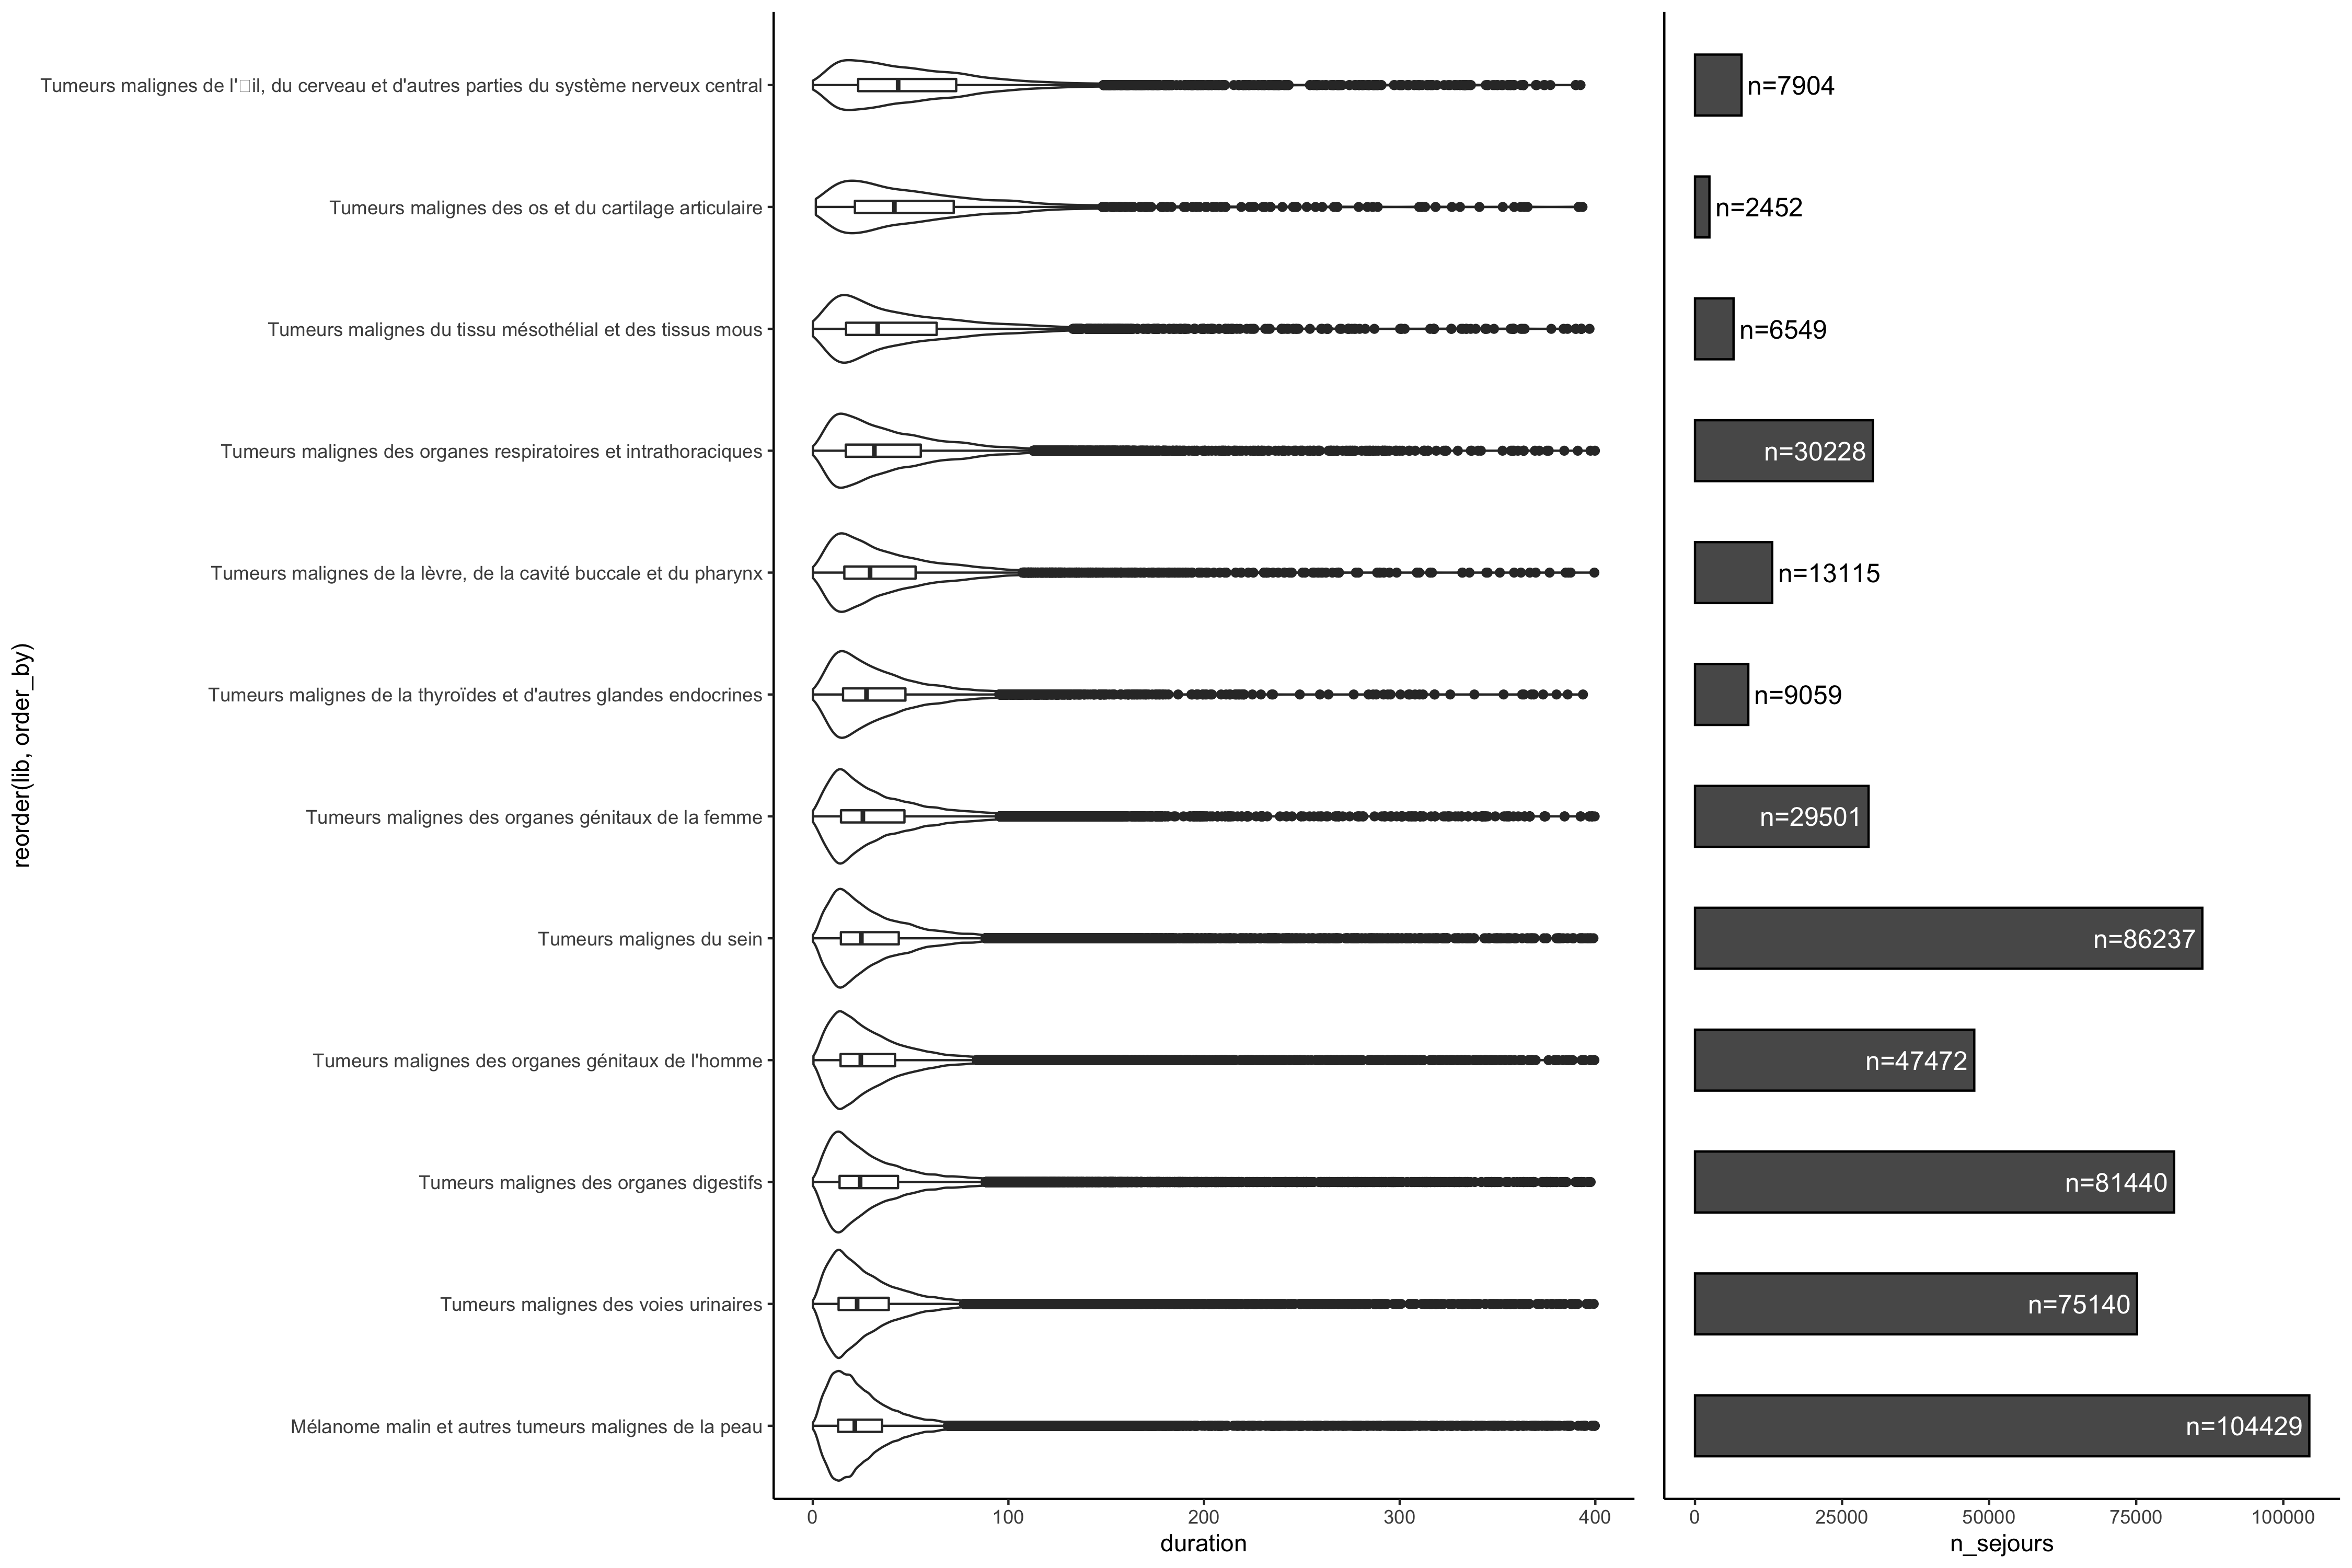
\includegraphics[width=0.9\textwidth]{images/routes/fig8_top.png}
    \centering
    \caption{ \textbf{Travel duration per cancer type.} Nice plot. }
    \label{fig:travel-duration-cancer-type}
\end{figure}

We also looked at the travel duration based on the
visited hospital. To assess the oncology specialization of the hospitals, we
used the hospitals clusters defined in (63). Only the hospitals from clusters 1
to 4 can perform cancer surgeries. Hospitals from clusters 1 and 2 are the most
specialized oncology hospitals, with all the key services such as cancer
surgery, radiotherapy, and chemotherapy. They also have the largest surgeries
volumes and are often specialized in even the rarest cancer types. Such
hospitals are sparsely located, and often placed in large cities. The hospitals
from clusters 3 and 4 are less specialized and are in both large cities and
sub-urban areas. The patients' travels were longer when they visit more
specialized hospitals from clusters 1 and 2. This might be explained by either
the need for more specialized care, or by the reputation of the hospital and the
incentive of going there in-stead of a smaller but closer hospital. We are now
interested in the spatial distribution of the patients travel duration, in
metropolitan France. On \cref{fig:routes-duration-france}, we showed the average
driving duration per municipalities on a map (A). Municipalities are filled by
duration bins. Unsurprisingly, median travel duration is short-ed for patients
living in dense municipalities. The median duration for patients living in
municipalities with more than 200 inhabitants per km\textsuperscript{2} is 16.4
minutes. However, for patients living in municipalities with less than 30
inhabitants per km\textsuperscript{2}, the median duration is 50.7 minutes,
about three times higher. Most patients living in dense areas can reach
hospitals from the more specialized clusters in little time. However, travel
durations are highest for patients from rural areas reaching the most
specialized hospitals (C).

\begin{figure}[h]
    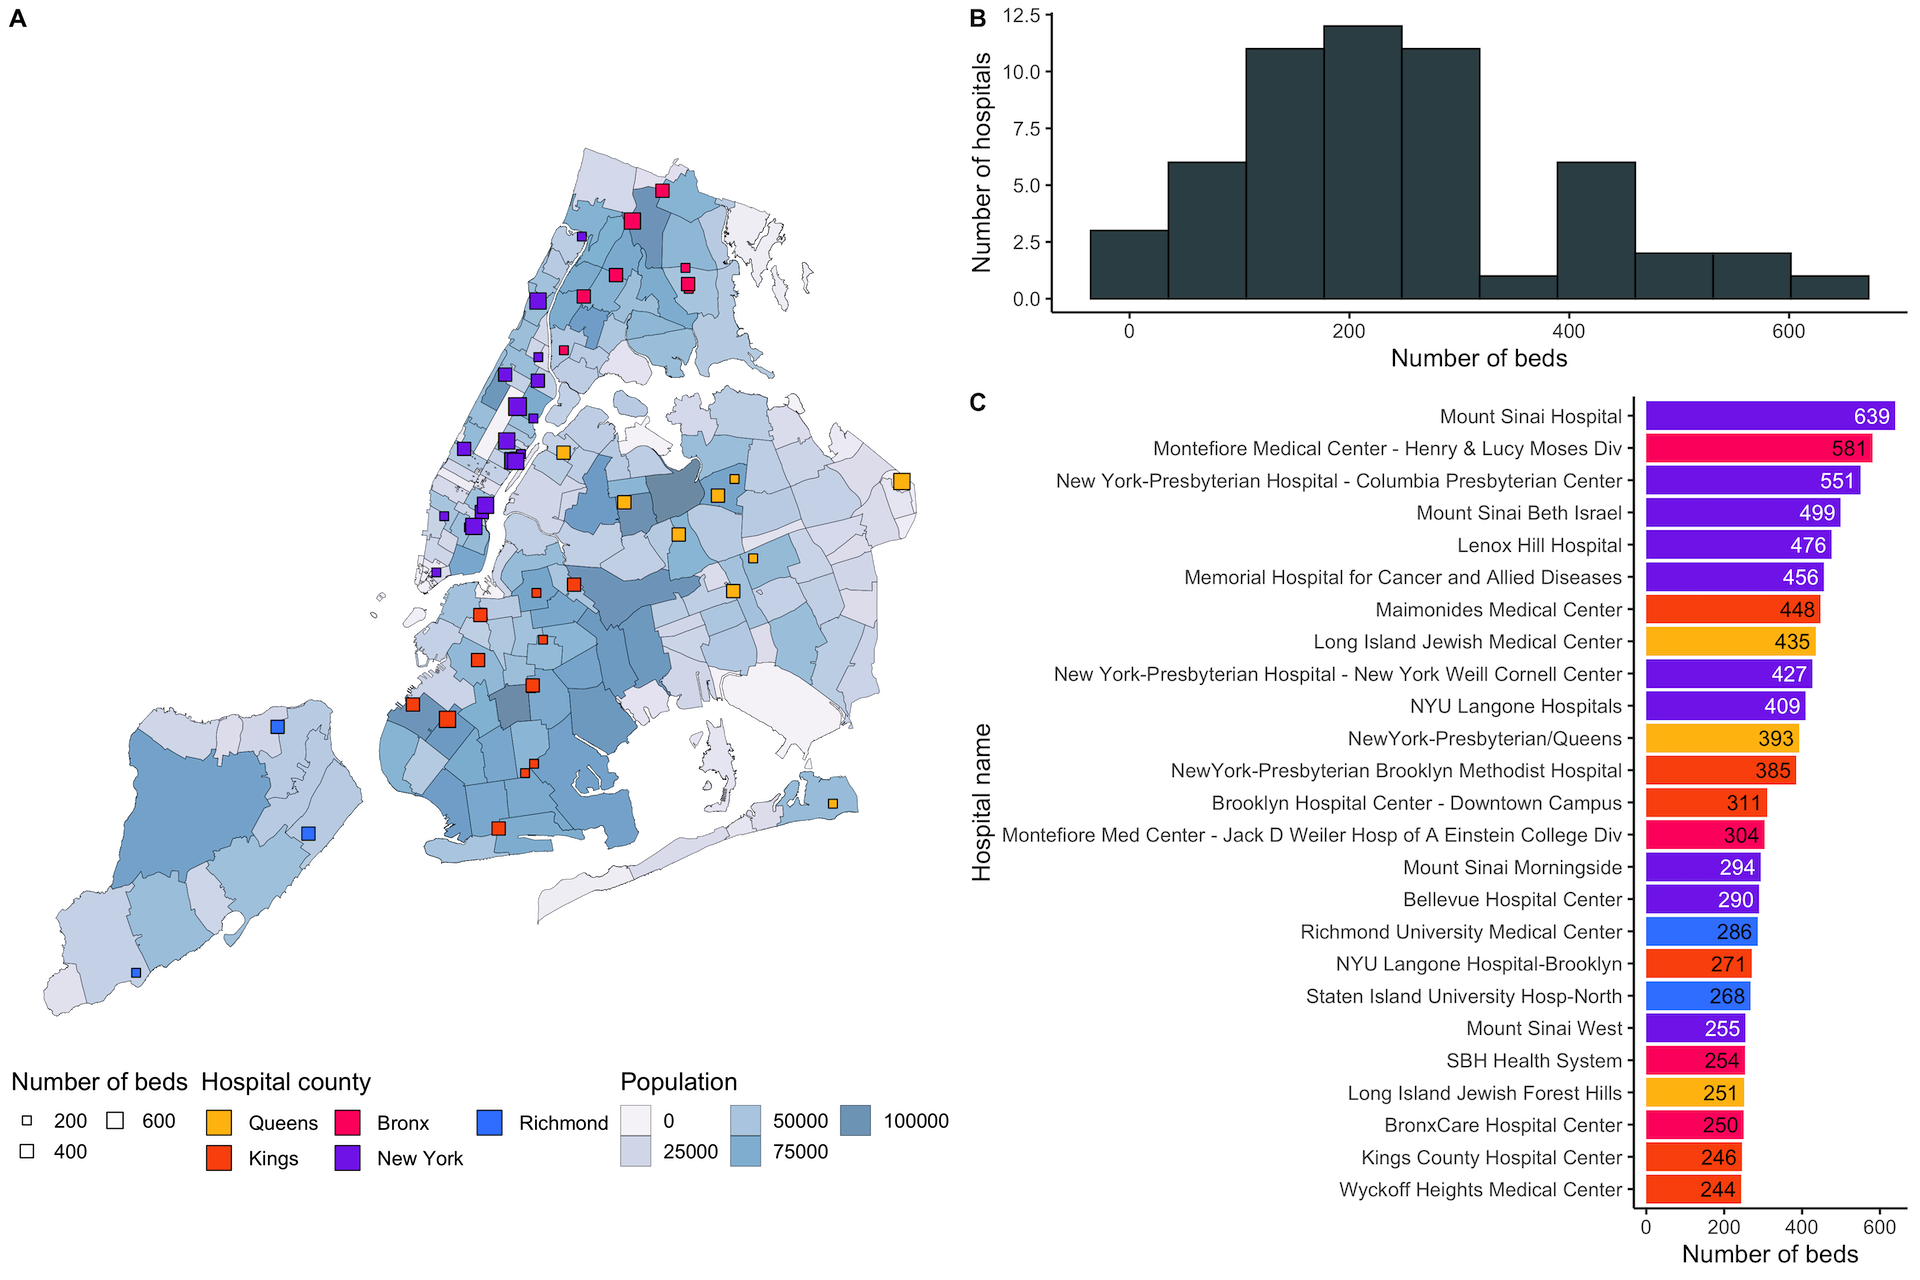
\includegraphics[width=0.9\textwidth]{images/routes/fig1.png}
    \centering
    \caption{ \textbf{Average driving duration for cancer patients in
            metropolitan France.} Map (A) displays the average driving duration by
        municipalities. The median travel duration is higher for municipalities
        with lower population densities (B). The median travel duration is
        especially high for patients from rural areas visiting specialized
        hospitals (C). Patients living in dense areas do not need to travel far
        when reaching specialized hospitals (C). }
    \label{fig:routes-duration-france}
\end{figure}

\subsection{Travel burden index}

While travel duration is a good proxy for the patients travel burden, it is not
the only contributor. In this section, we show the results of our travel burden
score.

\begin{figure}[h]
    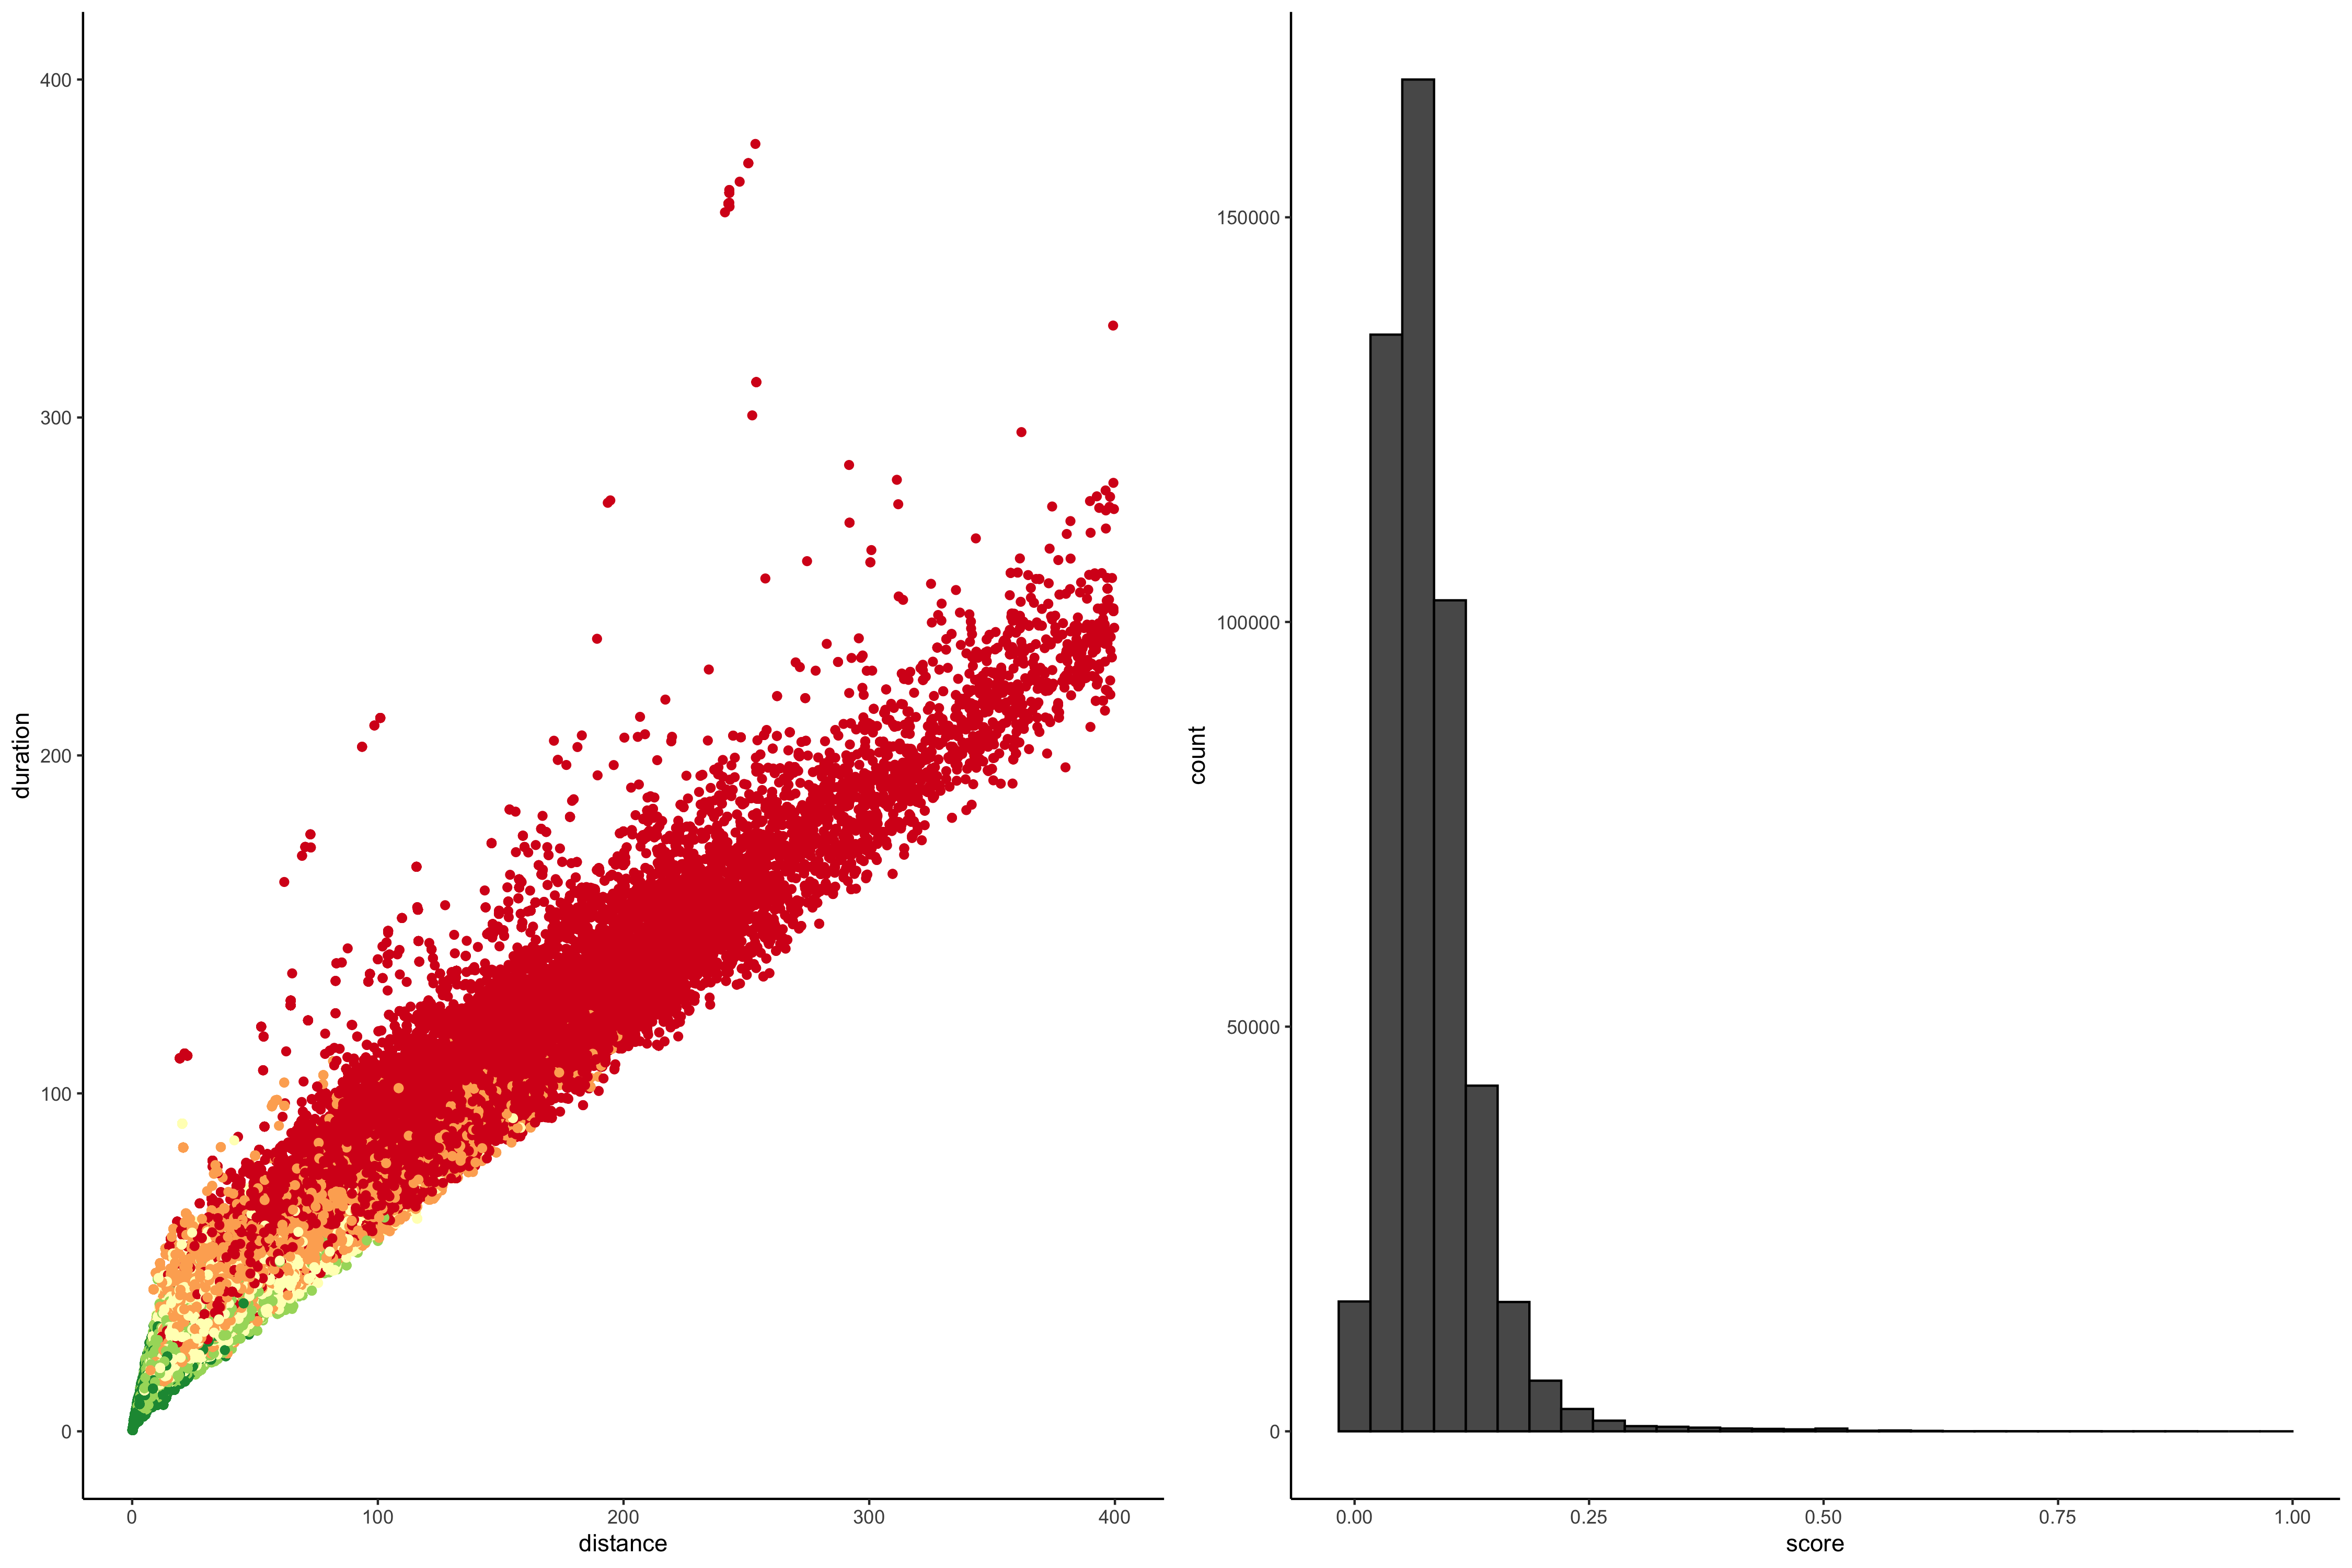
\includegraphics[width=0.9\textwidth]{images/routes/fig8_bottom.png}
    \centering
    \caption{ \textbf{Travel burden score histogram.} Nice plot. }
    \label{fig:travel-burden-histogram}
\end{figure}

On \cref{fig:routes-burden-index}, map (A) shows the spatial
distribution of the travel burden score. We display the average travel burden
score per municipality. The lower the score, the lower the travel burden is. We
discretized the average score into 5 quantiles. For municipalities in the first
quantile, the average travel burden score is in the top 20\%, meaning that
patients travel are shorts and road sinuosity is low. The first quantile is
colored in dark green on the map. The last quantile is where travel burden score
is the highest, and these municipalities are colored in pale yellow.
Municipalities with lower population densities have a higher proportion of
routes with high travel burden. For instance, among all the municipalities with
population densities lower than 30 inhabitants per km\textsuperscript{2} 47.5\%
are in the worst quantile, compared to only 19.8\% for municipalities with 200
or more inhabitants per km\textsuperscript{2} (B). We now compare the travel
burden score with several variables, such as duration, distance, sinuosity,
number of roundabouts, as well as the road type ratio (C). Higher travel burden
is associated with higher road sinuosity, distance, duration, as well as higher
number of roundabouts. The percentage of highway roads is also the highest in
this quantile.

\begin{figure}[h]
    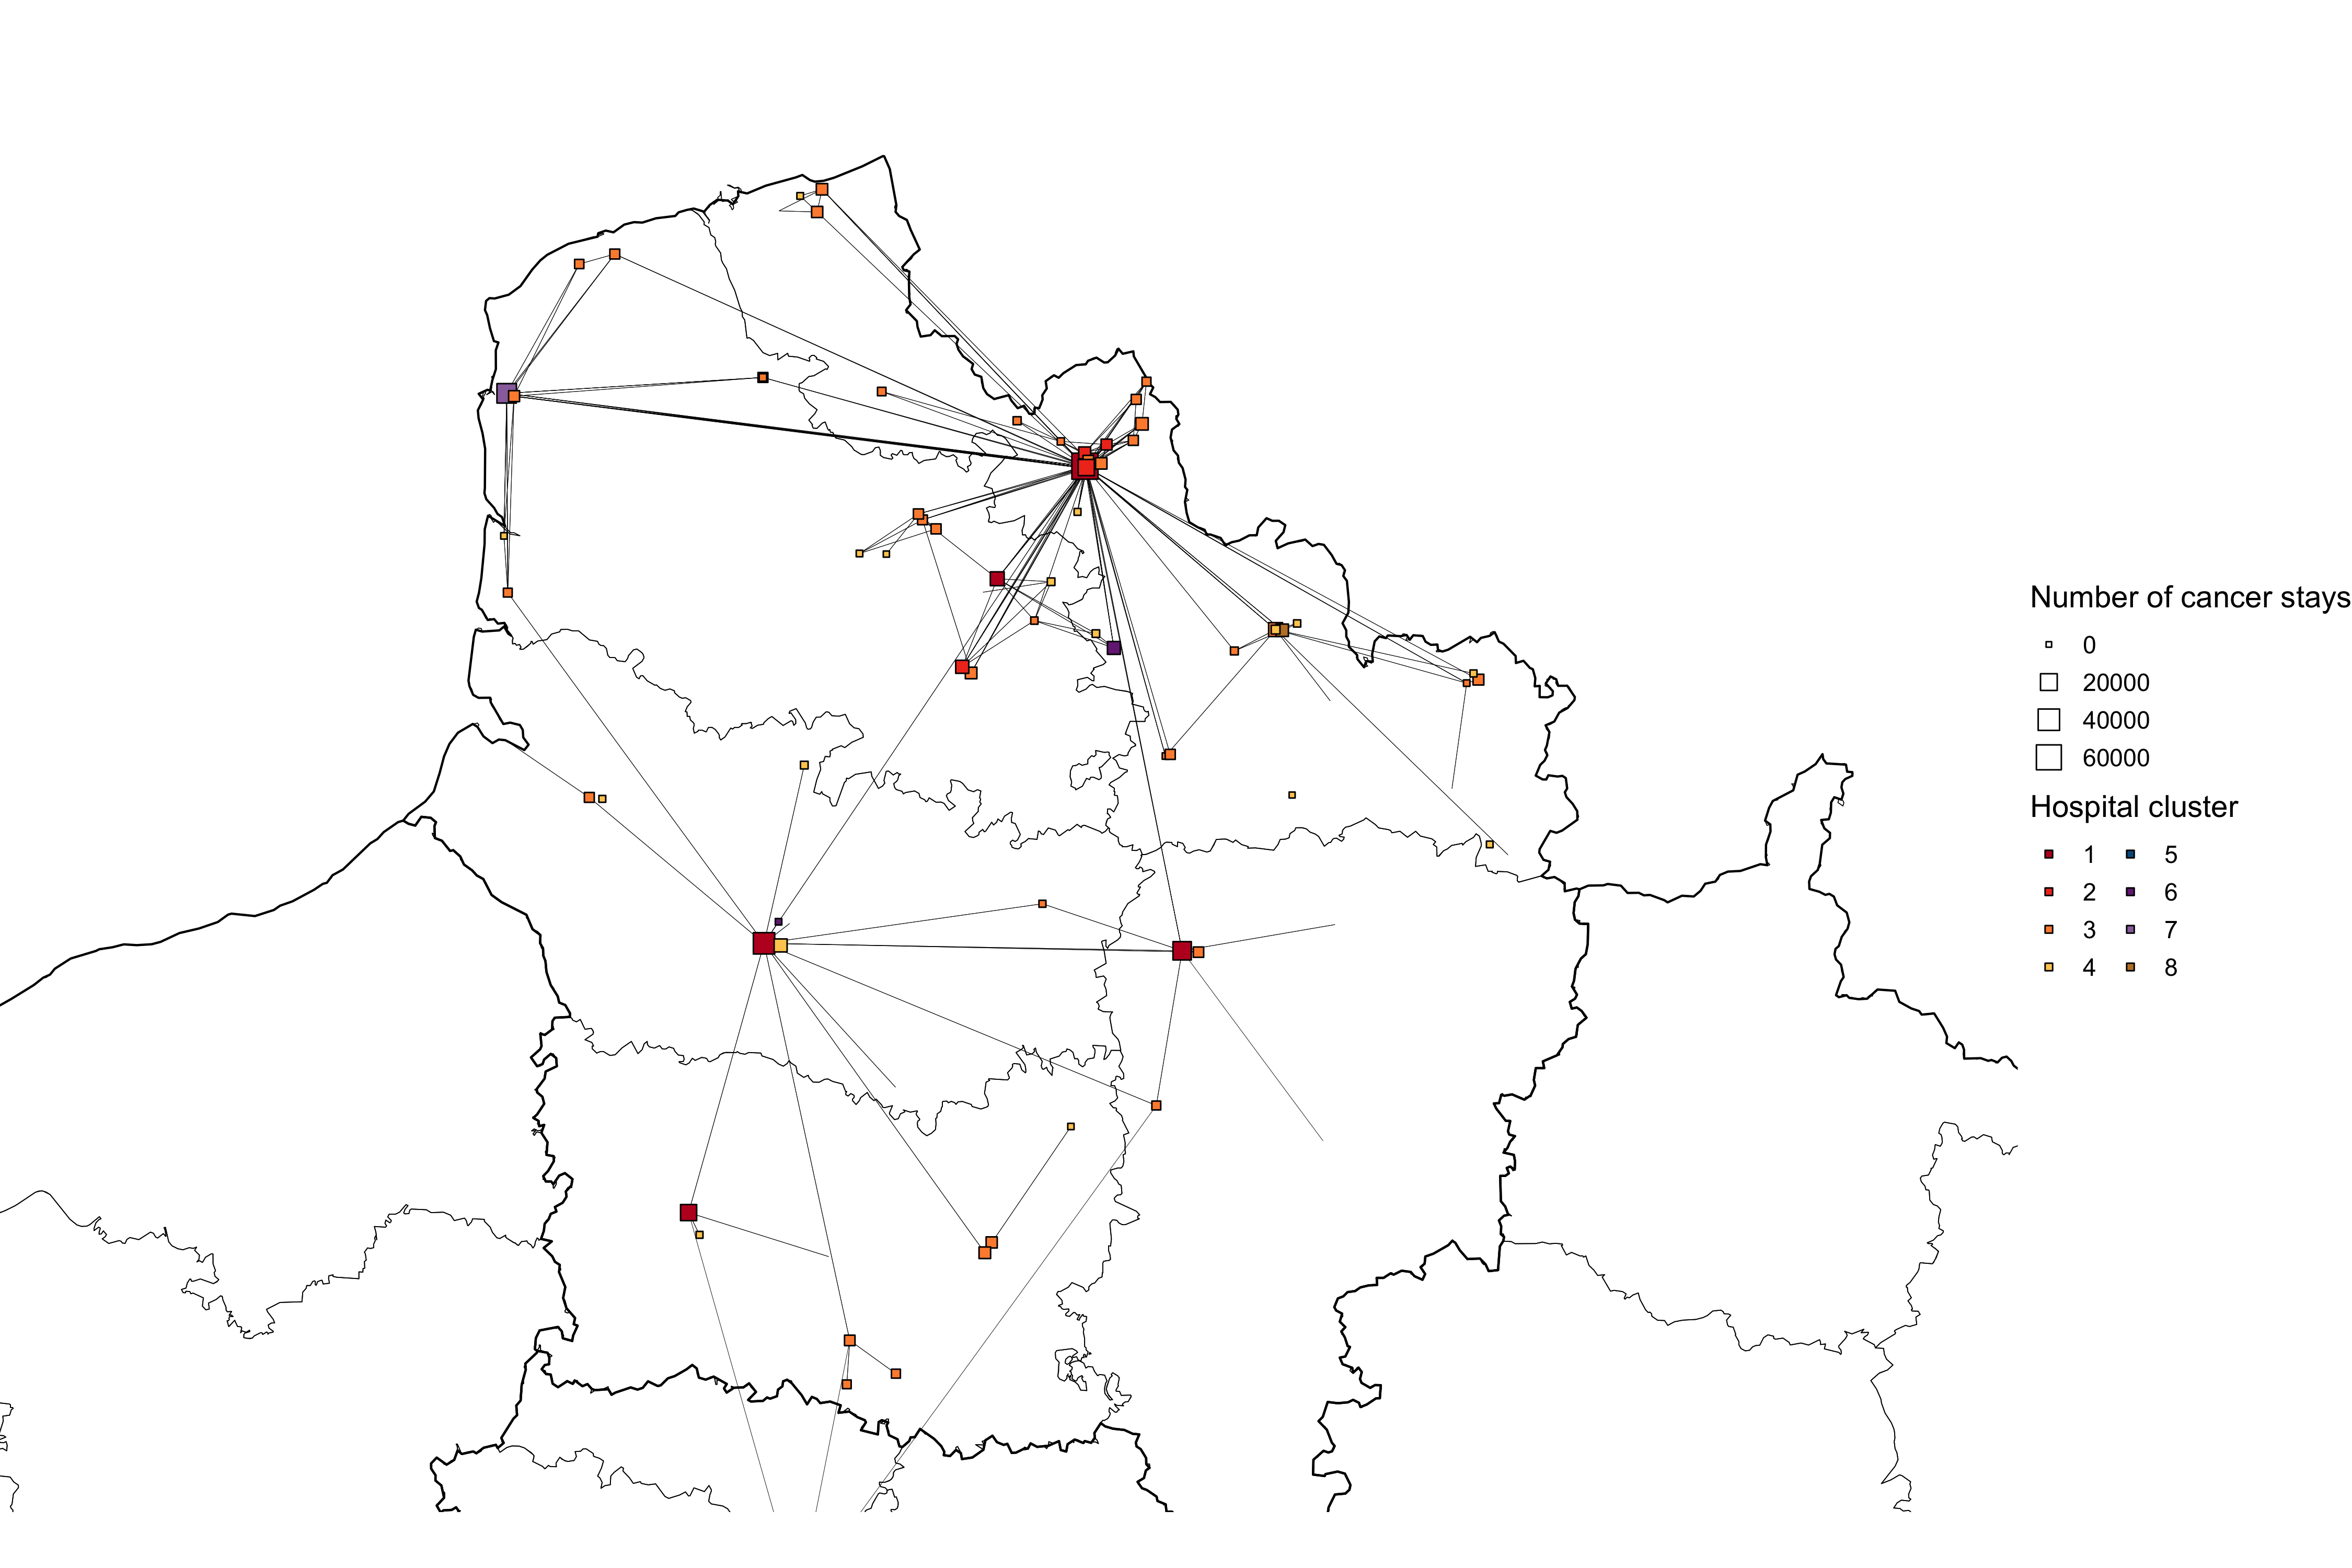
\includegraphics[width=0.9\textwidth]{images/routes/fig2.png}
    \centering
    \caption{
        \textbf{Travel burden index in metropolitan France.}
        The travel burden index is a composite score based on route duration,
        distance, number of roundabouts and sinuosity. The higher the score is,
        the more tedious the route is. The score distribution is displayed on
        map (A). The percentage of routes with higher scores increases in lower
        density areas (B). Figure (C) displays the input variables median values
        by score quantiles. For instance, the median road sinuosity is much
        higher when the score is high. }
    \label{fig:routes-burden-index}
\end{figure}

Now focusing on a single region.

\begin{figure}[h]
    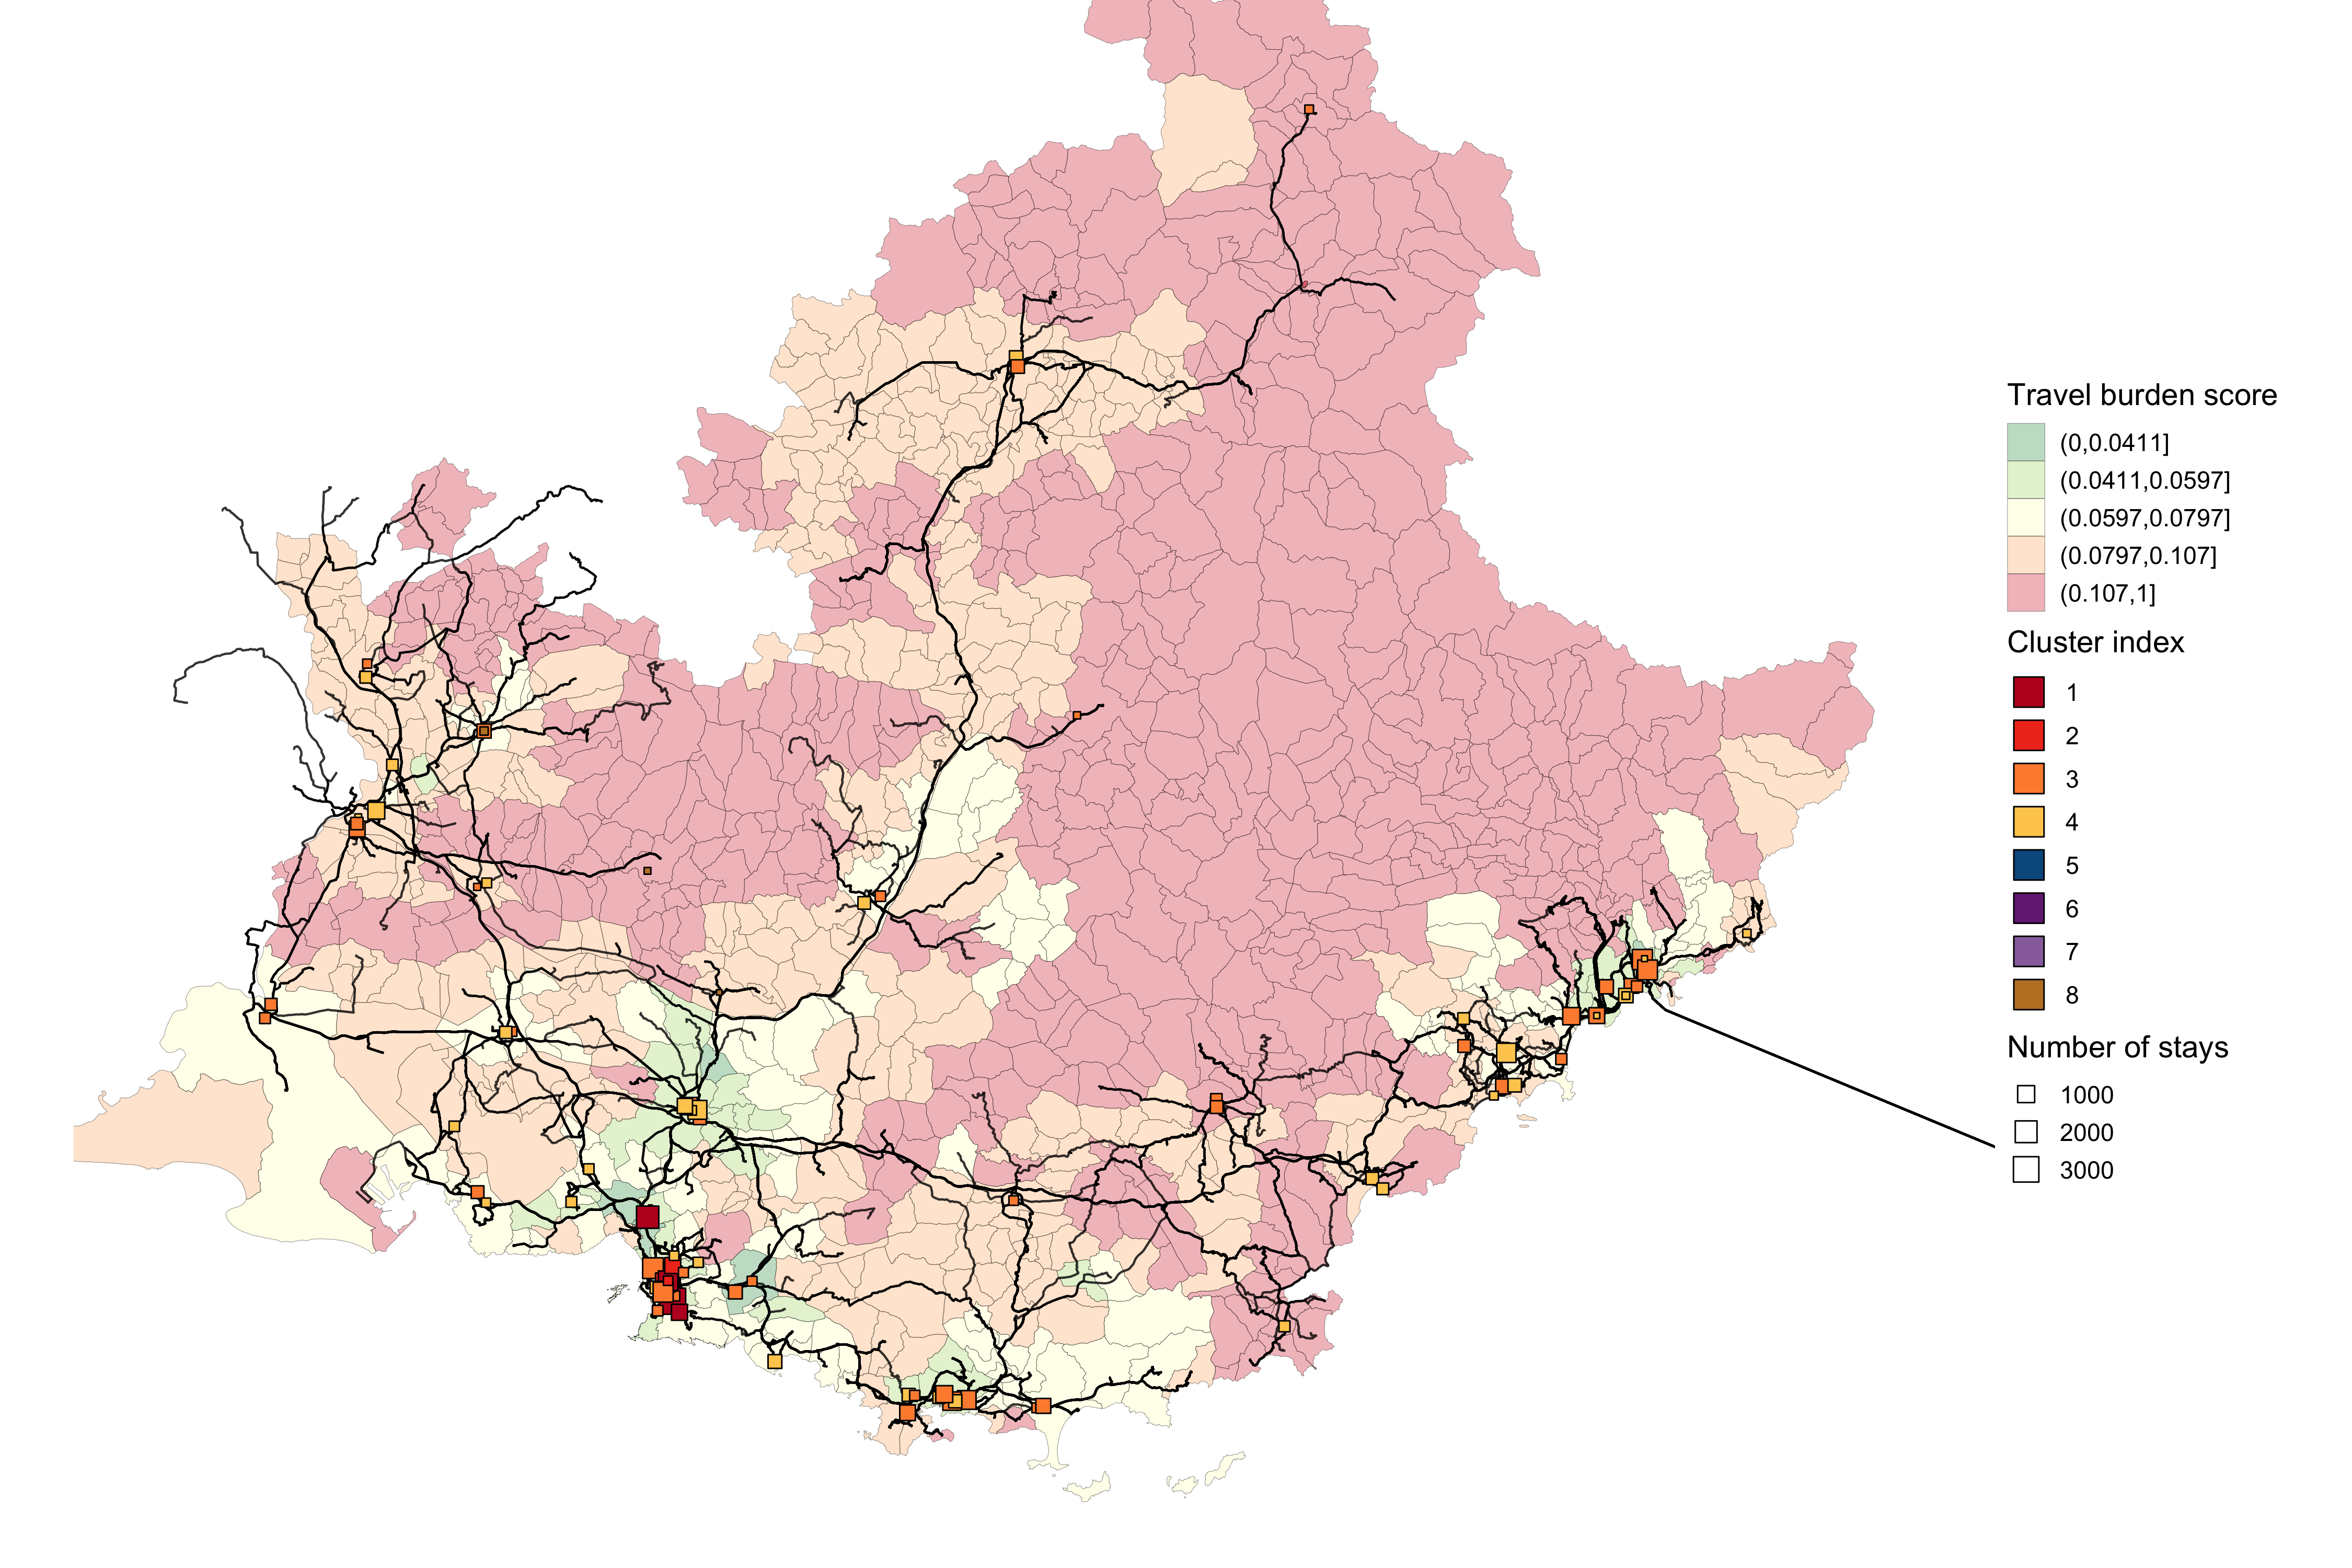
\includegraphics[width=0.9\textwidth]{images/routes/fig_7.png}
    \centering
    \caption{ \textbf{Travel burden score in PACA region.} Nice plot. }
    \label{fig:travel-duration-cancer-type}
\end{figure}

\subsection{Carbon footprint of patients travel}

We finally look at the carbon footprint of patients' travels on
\cref{fig:routes-co2-emissions}. Since we only considered direct emissions, the
carbon footprint is proportional to the traveled distance. The alluvium chart on
sub-figure (A) displays the number of patients routes between municipalities on
the left and hospitals on the right, in the Ain department, located in
Auvergne-Rhone-Alpes region. This department mostly hosts rural municipalities.
The alluvium flows are sized by number of stays and colored by the stays carbon
footprint. The darker flows indicate higher \ac{co2} emissions. We point that
the routes with the more emissions are not necessarily the routes with the most
patients. To illustrate this, we focus on the Bourg-en-Bresse city, which is the
largest city from the Ain department. On plot (B) we show the total \ac{co2}
emissions per visited hospital, for patients living in Bourg-en-Bresse.
Centre-Hospitalier de Fleyriat is the most visit-ed hospitals among patients
living in Bourg-en-Bresse, with 150 stays and 4-kilometer distance between the
municipality centroid and the hospital. The resulting \ac{co2} emissions are 72
kg. However, some patients are traveling outside of Bourg-en-Bresse to reach
hospitals based in Lyon, which represents at least an 80 km drive. For instance,
there were 18 stays in Hospital Lyon Sud, located at 91 km from Bourg-en-Bresse.
The resulting \ac{co2} emissions were 184 kg, which is more than twice the
emissions of the 150 stays in CH Fleyriat.

\begin{figure}[H]
    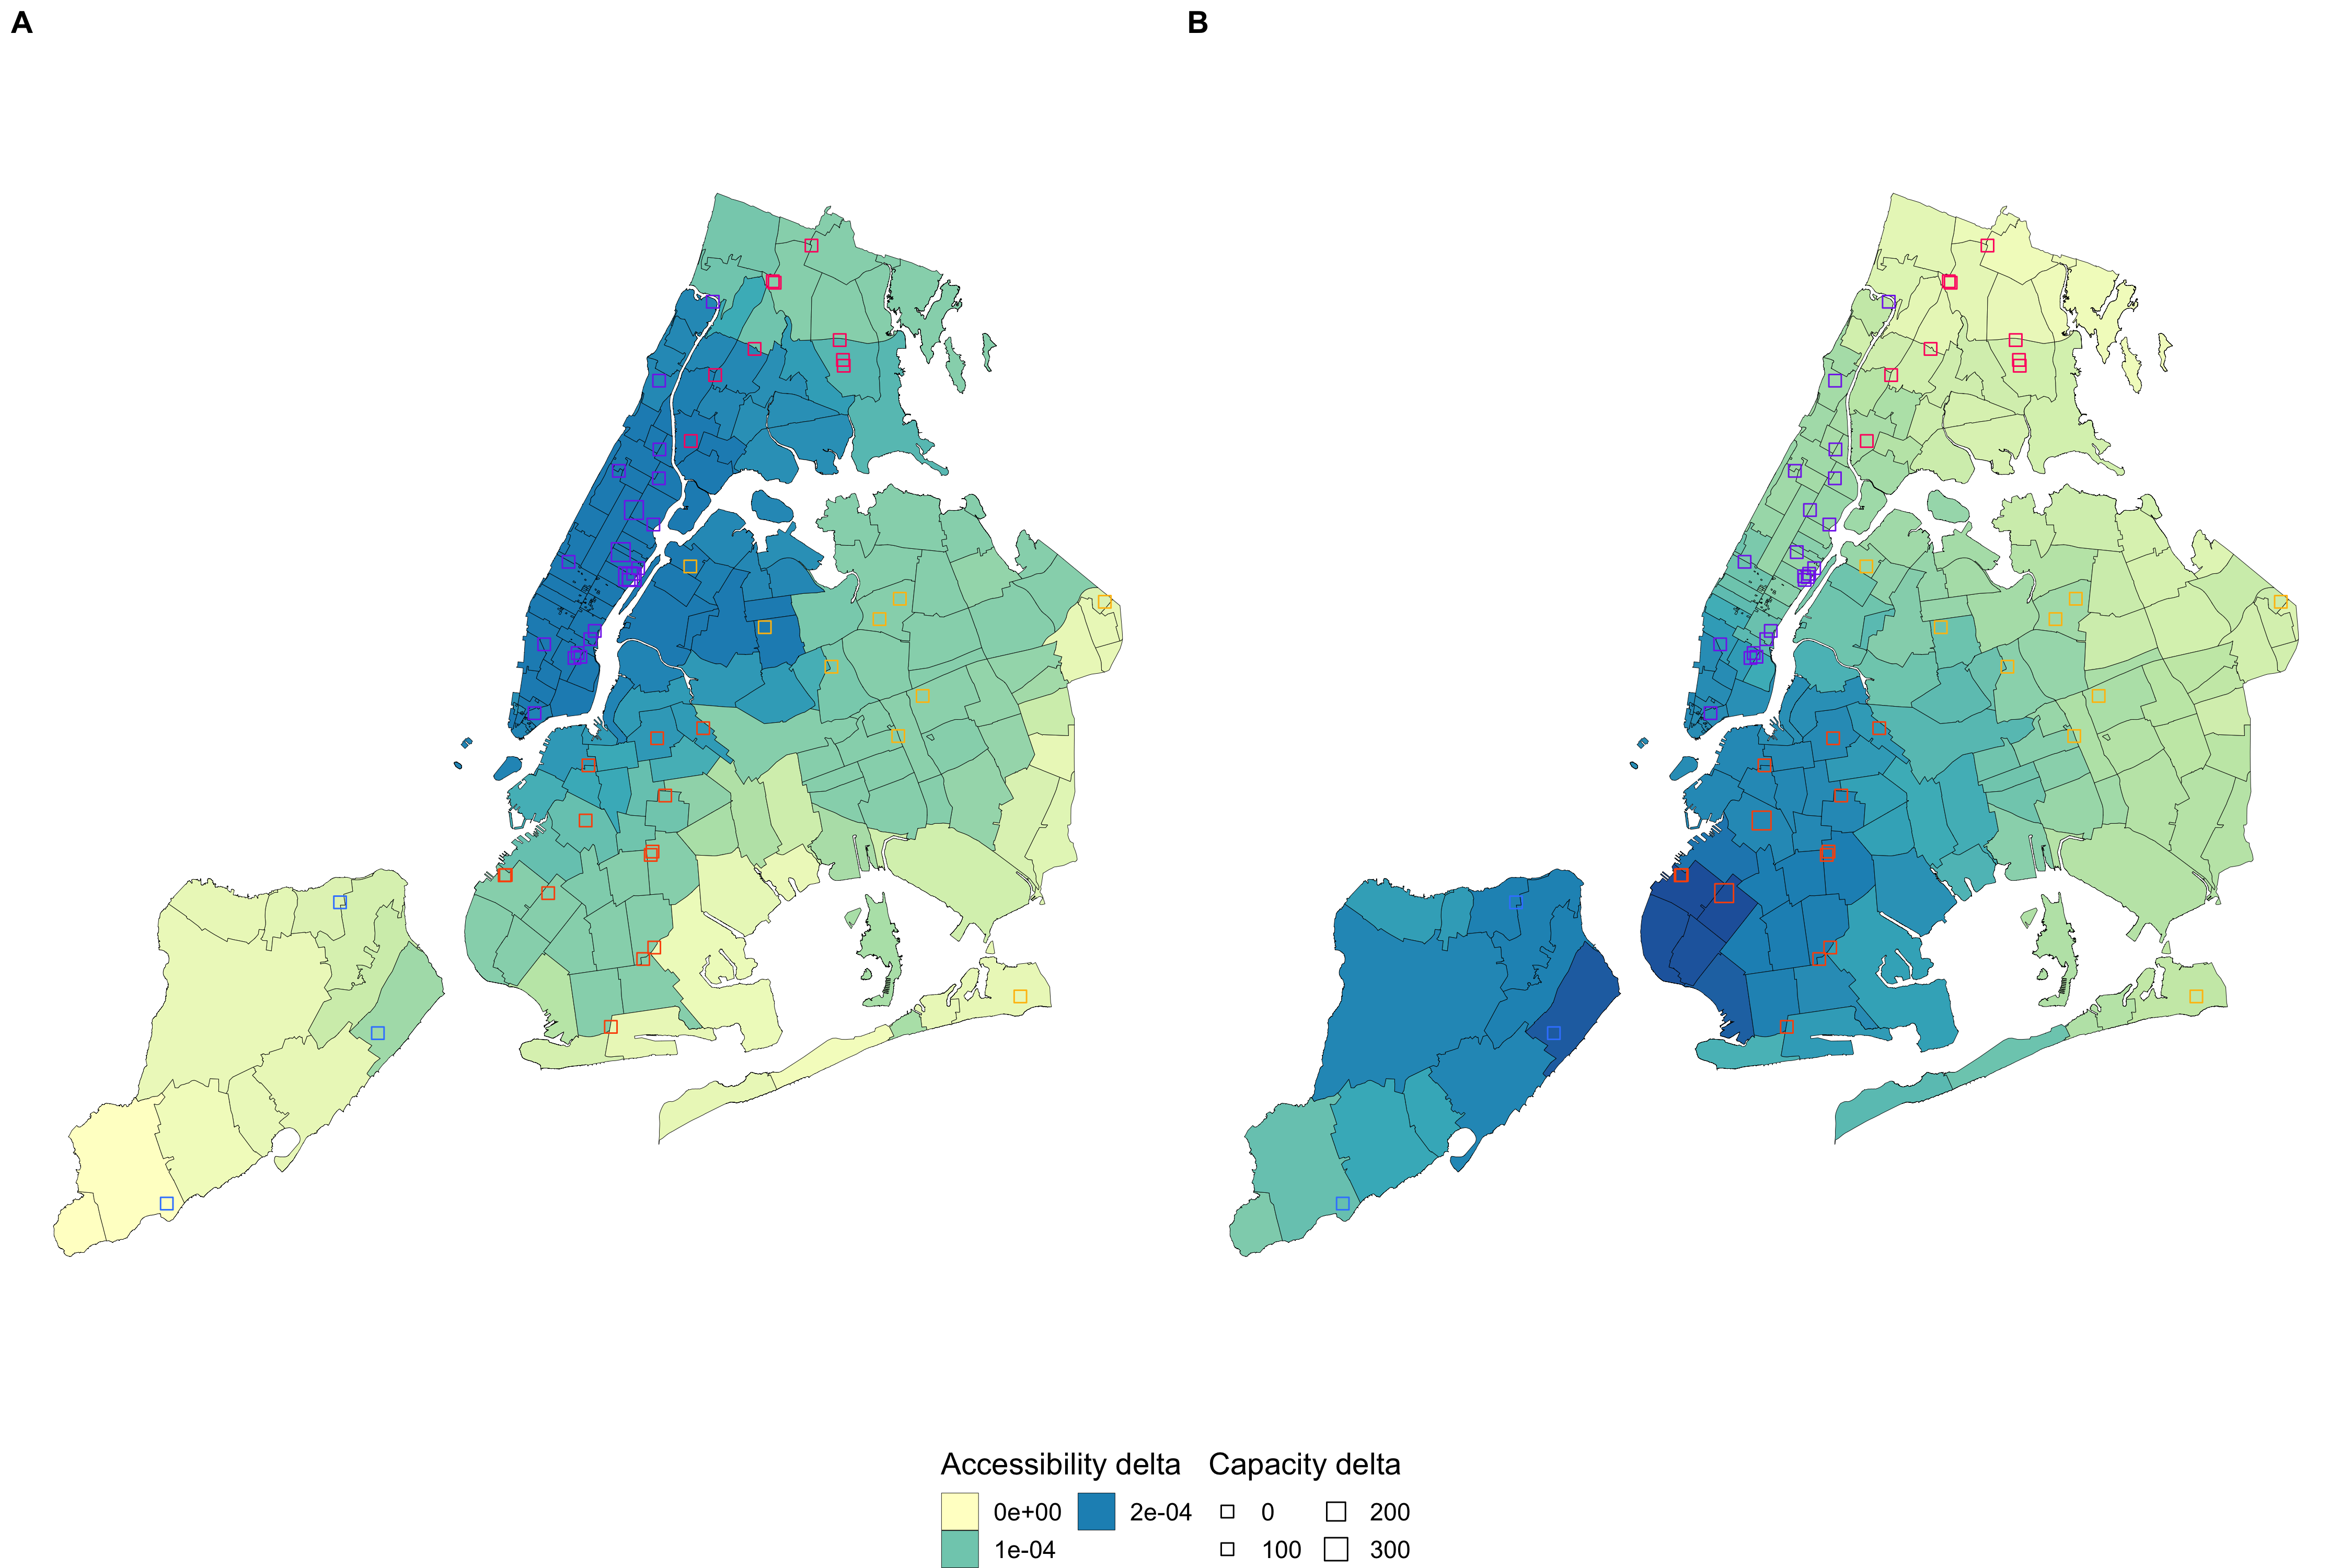
\includegraphics[width=0.9\textwidth]{images/routes/fig3.png}
    \centering
    \caption{ \textbf{\ac{co2} emissions for cancer patients travels} The
        \ac{co2} emissions are computed based on the GPS distance between the
        patient municipality centroid and hospital location. The total emission
        for a single travel is computed as the product of the average \ac{co2}
        emissions per km and the distance. Figure (A) displays the travels
        between municipalities in Ain department. Municipalities are on the
        left, hospitals on the right. Flows are sized by number of travels and
        colored by \ac{co2} emissions. Figure (B) shows the \ac{co2} emissions
        compared with number of stays in Bourg-en-Bresse city (Ain). The
        \ac{co2} emissions are higher for the fewer patients who traveled
        outside of the city to reach more specialized care centers in Lyon. }
    \label{fig:routes-co2-emissions}
\end{figure}

\section{Discussion}

The results of the travel analysis for cancer patients in metropolitan France
concur with the effects of regionalization of care observed in the literature.
We report longer travels for patients living in rural areas. The hospitals
specialized in oncology tend to receive patients from more distant population
locations. Finally, patients with less frequent cancers are forced to travel
further due to the limited number of hospitals that can correctly treat these
pathologies. We introduced the travel burden score, a new metric to consider
when studying patients travels. This score is proportional to not only distance
and duration, but also road sinuosity and number of roundabouts. The last two
variables, which are not explicitly captured by distance and duration, could be
responsible of more tedious drives for the patients, especially when their
health conditions are deprived. In our estimation, the \ac{co2} emissions are
directly proportional to the traveled distance. We did not consider indirect
emissions linked to the transportation. Car was the only transportation mean we
used, and we assumed every patient traveled by car, which might over-estimate
the \ac{co2} emissions. More research is needed to include public transportation
such as train or subway. The larger share of carbon emissions for cancer
surgeries is covered by frequent cancers, that can be treated in many hospitals,
like breast cancer for instance. For such pathologies, a rethink of the
regionalization of care model might be needed. Patients from less dense
municipalities could be sent to closer regional hospitals if we make sure the
surgeons' expertise is good enough. Partnerships with larger and more
specialized hospitals could be created to spread the more up to date knowledge
outside the urban hospitals. However, this will be more complicated for rare
cancers, where expertise is scarce and concentrated in the larger hospitals. On
a carbon footprint perspective, we believe the lower number of concerned
patients makes it less of a priority.
